\section{Implementation}
The project repository containing all of the source code from the project can be found here~\cite{projectrepo}.

\subsection{Initial Plan for Testing}
Originally, the plan was to compare pathfinding between standard Unity and the ECS version as a new AI API by Unity allows ECS to interface with it. This was scrapped fairly early on as there was too little documentation on how the new AI API worked so I could not get anything to run properly. Instead, I moved on to a simpler test scenario with transform manipulation for visual effects. The original pathfinding code still exists in the project repository, but it is not used.

\subsection{Transform Management Using a Galaxy Simulation}
\subsubsection{Simulation Design}
The design of the simulation consists of two parts: 
\begin{enumerate}
    \item Spawning and distributing stars across the galaxy
    \item Making each star orbit around the center of the galaxy at a given speed
\end{enumerate}
Stars are spawned in a manner that results in larger densities of stars towards the center of the galaxy and lower densities towards the outer edges. This is handled by defining a number of orbit circles and the difference in radius between them. The same amount of stars are then spawned per orbit, although a small random value is applied so that the galaxy looks more noisy and not like a set of circles. The general pseudocode for the spawning process looks like this:

\begin{algorithmic}
\For {$i=0; i<numberOfOrbits; i++$}
    \For{$j=0; j<numberOfStars/numberOfOrbits; j++$}
         \State Spawn Star at galaxyPosition;
         \State Generate a random point at the edge of a unit circle;
         \State Create normalized direction from random point;
         \State Star.position = galaxyPosition +
         \State (direction * (i+1) * distanceBetweenOrbits * randomValue);
         \State Star.orbitSpeed = starDistanceToGalaxyCenter;
    \EndFor
\EndFor
\end{algorithmic}

After the spawning process, each star then orbits around the center of the galaxy with a speed that is relative to the distance between the star and the center of the galaxy. The orbit speed has to be variable as keeping it the same would make it look like there is static galaxy that simply rotates around. This is because there are no real physics at play here and only a calculation for translating position on the edge of a circle using angles. To provide an example: with a speed modifier of 1 a star at (0,0,1) and a star at (0,0,100) would have moved to (1,0,0) and (100,0,0) with a 180 degree angle change when the galaxy is perpendicular to the Y-axis. 

\subsubsection{The Representation of Stars and Post Processing Usage}
Each star makes use of the default sphere mesh in Unity in combination with a randomly selected material which supports GPU instancing. This should provide a more taxing (and visually interesting) environment compared to simply using two dimensional sprites. 

Only having a large amount of differently coloured spheres would not look particularly appealing in a galaxy. This is why post processing bloom is applied in combination with HDR emission in the material of the stars to create a glowing appearance. As a result, the larger concentration of stars towards the center of the galaxy produces far more glow which provides a more visually natural image since stars actually emit light. The visual difference between not using and using bloom can be seen in Figure~\ref{fig:nobloom} and~\ref{fig:bloom}.
Multi-sampling anti aliasing (MSAA) is applied as it mitigates the flickering that comes from moving objects with bloom(TODO: Does this need citation? It's mostly just an artifact of Unity's bloom implementation). Finally, temporal anti aliasing (TAA) is applied to smoothen the final image. 

\begin{figure}[tbph]
    \centering
    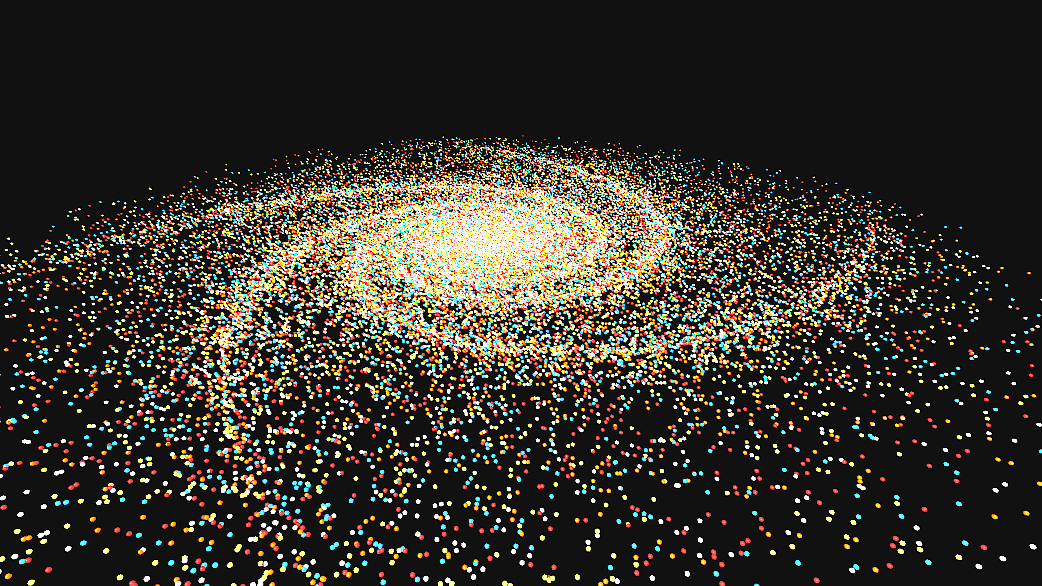
\includegraphics[width=1\textwidth]{Figures/noBloom.png}
    \caption[Galaxy without bloom]{The appearance of the simulated galaxy without any bloom}
    \label{fig:nobloom}
\end{figure}

\begin{figure}[tbph]
    \centering
    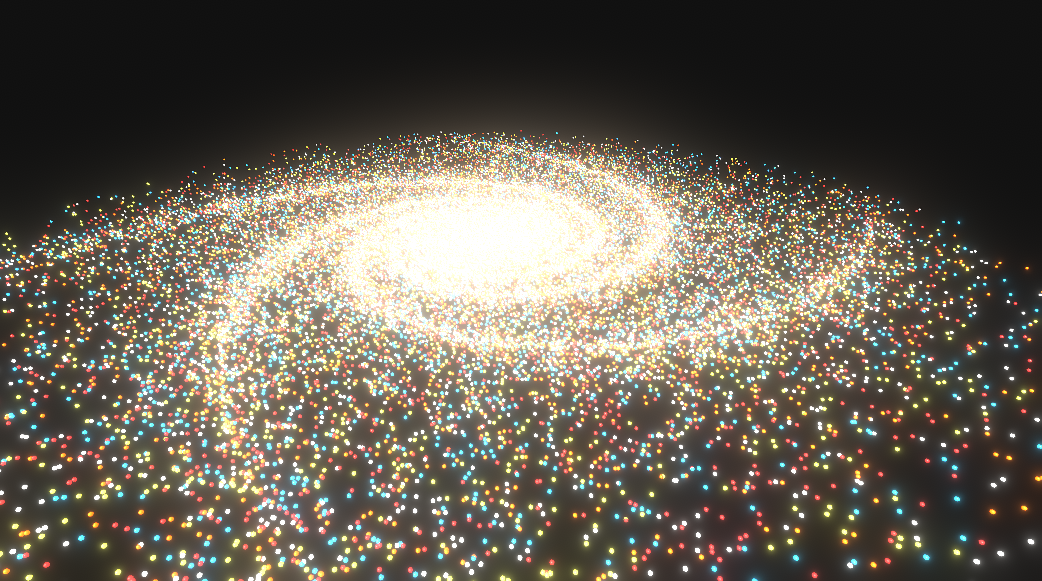
\includegraphics[width=1\textwidth]{Figures/bloom.png}
    \caption[Galaxy with bloom]{The appearance of the simulated galaxy with bloom}
    \label{fig:bloom}
\end{figure}

\subsubsection{Naive Unity Implementation}
The naive Unity implementation is split in two source files: StarSpawner.cs~\cite{naiveSpawner} and OrbitAroundTransform.cs~\cite{naiveOrbiter}. The former takes care of spawning stars from a provided prefab in a similar vein to the previously mentioned pseudocode. The latter script is attached to every single star and consists of a target to orbit around, the axis that the rotation makes use of and the speed of rotation. This script also has a Update() method which rotates the star around the center of the galaxy using Unity's RotateAround() function~\cite{rotateAroundFunction}.

This is more or less the simplest implementation I think of, hence the naming of the case. Since each star has a script attached which inherits from Unity's MonoBehaviour class, the performance of this test case is expected to be rather low.

\subsubsection{Job Optimised Unity Implementation}
The job optimised counterpart to the naive Unity implementation consists of one source file: GalaxyManager.cs~\cite{jobOptimizedManager}. The script takes care of both spawning and translating the stars around. This means that each star does not contain any behaviour by itself and everything is managed in one script that exists in one instance. 

The process of spawning stars is more or less the same as with the naive implementation, although the distance between the star and the center of the galaxy is stored for later usage. 

The process of translating stars is handled by using a job from the new Job System that Unity introduced together with ECS and the Burst compiler. This is a ParallelFor-style job, meaning that it will split the loop among all available worker threads. The job is designed to be similar with how Unity's RotateAround() function~\cite{rotateAroundFunction} is in terms of usage, although it does not change any rotation matrices. One thing to note about the Job System is that all data that is used should be declared and provided ahead of time so the job can execute it in a native environment. Due to this, there is some additional boilerplate code in this test case so that all important data can be stored and transferred over to the job. 

The means of translating a star along its own orbit is handled by first finding the current angle between the star and the center of the galaxy. This angle is then subtracted from with Time.deltaTime multiplied by the speed of the star. Standard trigonometry functions like cosine and sine are used together with the new angle to update the position of the star relative to the galaxy center. Finally, the star is offset so that it keeps the distance from the center which was stored during spawning. 

\subsubsection{Naive ECS Implementation}
The ECS implementation is split up into a variety of files and the general pipeline is fairly different from standard Unity. This section is mostly focused on the specific implementation in this case so some technical background in ECS might be useful to understand the source code. 

\paragraph{Components and Bootstrapping}
Since the galaxy simulation only consists of stars there only is one component. This can be seen in the TransformOrbitComponents.cs script~\cite{transformOrbitComponent} where the OrbitingStar component only stores the necessary data for orbiting. Entity creation is handled in a bootstrapper script~\cite{bootstrapper} which consumes galaxy settings from a GameObject in the scene and creates entities that consist of four components. These four components are Position, Scale, OrbitingStar and a MeshInstanceRenderer. During creation of entities, each star is placed around in the galaxy similar to how the other test cases handle it. 

\paragraph{Systems}
This implementation only consists of one system which is found in StarOrbitSystem.cs~\cite{orbitSystem}. The algorithm for translation is mostly the same as in the job optimised Unity case although there is a difference in how data is acquired. This is handled with a IJobProcessComponentData$<$...$>$-style job which specifically works with ECS components. Providing component types as parameters to this interface results in the job filtering all entities based on the provided input. In this case, the job acquires all entities that contain a Position and OrbitingStar component and handles translation of these. 
